\section{Приложение}

\subsection{Приложение 1} \label{Приложение 1}
Схемы экспериментальных установок для двух методов измерения скорости звука приведены на рис. 2 и 3.
\begin{figure}[ht]
    \label{figure2}
    \center{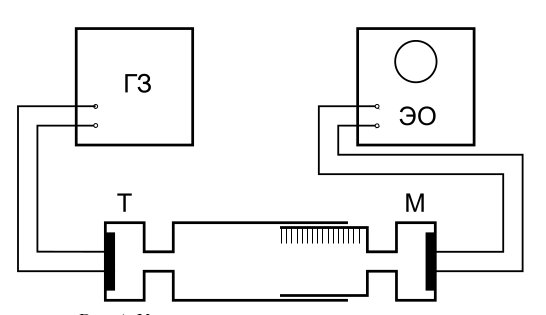
\includegraphics[scale=0.5]{img/exp-ust1.png}}
    \caption{Экспериментальная установка для измерения cкорости звука при помощи раздвижной трубы}
\end{figure}
\begin{figure}[ht]
    \label{figure3}
    \center{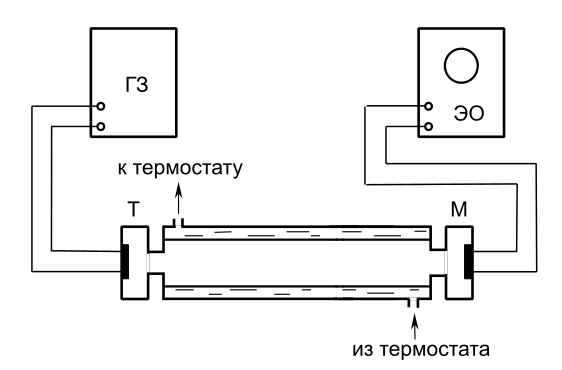
\includegraphics[scale=0.5]{img/exp-ust2.png}}
    \caption{Экспериментальная установка для измерения cкорости звука при помощи трубы постоянной длины}
\end{figure}

В обеих установках звуковые колебания возбуждаются телефоном \text{Т} и улавливаются микрофоном \text{М}. Мембрана телефона приводится в движение переменным током звуковой частоты, в качестве источника переменной ЭДС используется звуковой генератор \text{ГЗ}. Возникающий в микрофоне сигнал наблюдается на осциллографе \text{ЭО}. Микрофон и телефон присоединены к установке с помощью тонких резиновых трубок. Первая установка (рис. 1) содержит раздвижную трубу с миллиметровой шкалой. Через патрубок труба наполняется воздухом. Вторая установка содержит теплоизолированную трубу постоянной длины. Воздух в трубе нагревается водой из термостата. Температура воздуха равна температуре воды в термостате.

\subsection{Приложение 2} \label{Приложение 2}
\begin{table}[h]
    \centering
    \begin{tabular}{|c|c|c|}
    \hline
    $k$ & $L_{n+k} - L_n, \text{м}$ & $\sigma_L, \text{м}$  \\ \hline
    1   & 0.031                     & 0.005  \\ \hline
    2   & 0.118                     & 0.005  \\ \hline
    3   & 0.203                     & 0.005  \\ \hline
\end{tabular}
    \caption{Зависимость удлинения $L_{n+k} - L_n$ трубы от номера резонанса $k$ при частоте звуковой волны $f = 2\text{КГц}$, $\sigma_L$ - погрешность измерения удлинения трубы}
    \label{tab:t1}
\end{table}

\begin{table}[h]
    \centering
    \begin{tabular}{|c|c|c|}
    \hline
    $k$ & $L_{n+k} - L_n, \text{м}$ & $\sigma_L, \text{м}$  \\ \hline
    1   & 0.004                     & 0.005  \\ \hline
    2   & 0.062                     & 0.005  \\ \hline
    3   & 0.119                     & 0.005  \\ \hline
    4   & 0.177                     & 0.005  \\ \hline
\end{tabular}
    \caption{Зависимость удлинения $L_{n+k} - L_n$ трубы от номера резонанса $k$ при частоте звуковой волны $f = 3\text{КГц}$, $\sigma_L$ - погрешность измерения удлинения трубы}
    \label{tab:t2}
\end{table}

\begin{table}[h]
    \centering
    \begin{tabular}{|c|c|c|}
    \hline
    $k$ & $L_{n+k} - L_n, \text{м}$ & $\sigma_L, \text{м}$  \\ \hline
    1   & 0.034                     & 0.005  \\ \hline
    2   & 0.077                     & 0.005  \\ \hline
    3   & 0.121                     & 0.005  \\ \hline
    4   & 0.162                     & 0.005  \\ \hline
    5   & 0.207                     & 0.005  \\ \hline
\end{tabular}
    \caption{Зависимость удлинения $L_{n+k} - L_n$ трубы от номера резонанса $k$ при частоте звуковой волны $f = 4\text{КГц}$, $\sigma_L$ - погрешность измерения удлинения трубы}
    \label{tab:t3}
\end{table}

\begin{table}[h]
    \centering
    \begin{tabular}{|c|c|c|}
    \hline
    $k$ & $L_{n+k} - L_n, \text{м}$ & $\sigma_L, \text{м}$  \\ \hline
    1   & 0.016                     & 0.005  \\ \hline
    2   & 0.052                     & 0.005  \\ \hline
    3   & 0.086                     & 0.005  \\ \hline
    4   & 0.122                     & 0.005  \\ \hline
    5   & 0.156                     & 0.005  \\ \hline
    5   & 0.191                     & 0.005  \\ \hline
\end{tabular}
    \caption{Зависимость удлинения $L_{n+k} - L_n$ трубы от номера резонанса $k$ при частоте звуковой волны $f = 5\text{КГц}$, $\sigma_L$ - погрешность измерения удлинения трубы}
    \label{tab:t4}
\end{table}

\begin{table}[h]
    \centering
    \begin{tabular}{|c|c|c|}
    \hline
    $k$ & $L_{n+k} - L_n, \text{м}$ & $\sigma_L, \text{м}$  \\ \hline
    1   & 0.006                     & 0.005  \\ \hline
    2   & 0.036                     & 0.005  \\ \hline
    3   & 0.065                     & 0.005  \\ \hline
    4   & 0.094                     & 0.005  \\ \hline
    5   & 0.123                     & 0.005  \\ \hline
    5   & 0.151                     & 0.005  \\ \hline
\end{tabular}
    \caption{Зависимость удлинения $L_{n+k} - L_n$ трубы от номера резонанса $k$ при частоте звуковой волны $f = 6\text{КГц}$, $\sigma_L$ - погрешность измерения удлинения трубы}
    \label{tab:t5}
\end{table}
\newpage
\subsection{Приложение 3} \label{Приложение 3}

\begin{table}[h]
    \centering
    \begin{tabular}{|c|c|c|}
    \hline
    $k$ & $f_{k+1} - f_1, \text{Гц}$ & $\sigma_f, \text{Гц}$  \\ \hline
    1   & 232                        & 3  \\ \hline
    2   & 461                        & 3  \\ \hline
    3   & 691                        & 3  \\ \hline
    4   & 923                        & 3  \\ \hline
    5   & 1152                       & 3  \\ \hline
\end{tabular}
    \caption{Зависимость разности $f_{k+1} - f_1$ частот текущего и первого резонансов от номера резонанса $k$ при температуре воздуха $T = 21.7\celsius$, $\sigma_f$ - погрешность измерения частоты}
    \label{tab:t6}
\end{table}

\begin{table}[h]
    \centering
    \begin{tabular}{|c|c|c|}
    \hline
    $k$ & $f_{k+1} - f_1, \text{Гц}$ & $\sigma_f, \text{Гц}$  \\ \hline
    1   & 235                        & 3  \\ \hline
    2   & 468                        & 3  \\ \hline
    3   & 700                        & 3  \\ \hline
    4   & 935                        & 3  \\ \hline
    5   & 1168                       & 3  \\ \hline
\end{tabular}
    \caption{Зависимость разности $f_{k+1} - f_1$ частот текущего и первого резонансов от номера резонанса $k$ при температуре воздуха $T = 30.0\celsius$, $\sigma_f$ - погрешность измерения частоты}
    \label{tab:t6}
\end{table}

\begin{table}[h]
    \centering
    \begin{tabular}{|c|c|c|}
    \hline
    $k$ & $f_{k+1} - f_1, \text{Гц}$ & $\sigma_f, \text{Гц}$  \\ \hline
    1   & 236                        & 3  \\ \hline
    2   & 476                        & 3  \\ \hline
    3   & 711                        & 3  \\ \hline
    4   & 948                        & 3  \\ \hline
    5   & 1186                       & 3  \\ \hline
\end{tabular}
    \caption{Зависимость разности $f_{k+1} - f_1$ частот текущего и первого резонансов от номера резонанса $k$ при температуре воздуха $T = 40.0\celsius$, $\sigma_f$ - погрешность измерения частоты}
    \label{tab:t7}
\end{table}
\newpage
\begin{table}[h]
    \centering
    \begin{tabular}{|c|c|c|}
    \hline
    $k$ & $f_{k+1} - f_1, \text{Гц}$ & $\sigma_f, \text{Гц}$  \\ \hline
    1   & 242                        & 3  \\ \hline
    2   & 481                        & 3  \\ \hline
    3   & 723                        & 3  \\ \hline
    4   & 965                        & 3  \\ \hline
    5   & 1206                       & 3  \\ \hline
\end{tabular}
    \caption{Зависимость разности $f_{k+1} - f_1$ частот текущего и первого резонансов от номера резонанса $k$ при температуре воздуха $T = 50.0\celsius$, $\sigma_f$ - погрешность измерения частоты}
    \label{tab:t8}
\end{table}

\begin{table}[h]
    \centering
    \begin{tabular}{|c|c|c|}
    \hline
    $k$ & $f_{k+1} - f_1, \text{Гц}$ & $\sigma_f, \text{Гц}$  \\ \hline
    1   & 245                        & 3  \\ \hline
    2   & 488                        & 3  \\ \hline
    3   & 735                        & 3  \\ \hline
    4   & 980                        & 3  \\ \hline
    5   & 1215                       & 3  \\ \hline
\end{tabular}
    \caption{Зависимость разности $f_{k+1} - f_1$ частот текущего и первого резонансов от номера резонанса $k$ при температуре воздуха $T = 60.0\celsius$, $\sigma_f$ - погрешность измерения частоты}
    \label{tab:t9}
\end{table}
\newpage
\subsection{Приложение 4} \label{Приложение 4}

\begin{table}[h]
    \centering
    \begin{tabular}{|c|c|c|c|c|c|c|c|}
    \hline
    $\alpha, \text{м}$ & $f\cdot 10^{3}, \text{Гц}$ & $\lambda, \text{м}$ & $c, \frac{\text{м}}{\text{с}}$ & $\sigma_\alpha \cdot 10^{-3}, \text{м}$ & $\sigma_f, \text{Гц}$ & $\sigma_\lambda \cdot 10^{-3}, \text{м}$ & $\sigma_c, \frac{\text{м}}{\text{с}}$ \\ \hline
    0.086   & 2 & 0.172 & 344 & 0.58 & 3 & 1.16 & 2.34\\ \hline
    0.058   & 3 & 0.116 & 348 & 0.14 & 3 & 0.28 & 0.91\\ \hline
    0.043   & 4 & 0.086 & 344 & 0.30 & 3 & 0.60 & 2.41\\ \hline
    0.035   & 5 & 0.070 & 350 & 0.14 & 3 & 0.28 & 1.42\\ \hline
    0.029   & 6 & 0.058 & 348 & 0.14 & 3 & 0.28 & 1.69\\ \hline
\end{tabular}
    \caption{Зависимость скорости $c$ звука в воздухе от частоты $f$ звуковой волны. $\alpha$ - угловой коэффициент графика зависимости $(L_{n+k} - L_n)(k)$, $\lambda$ - длина волны, $\sigma_\alpha, \sigma_f, \sigma_\lambda, \sigma_c$ - погрешности измерения углового коэффициента, частоты, длины волны, скорости звука соответственно.}
    \label{tab:t10}
\end{table}

\subsection{Приложение 5} \label{Приложение 5}

\begin{table}[h]
    \centering
    \begin{tabular}{|c|c|c|c|c|c|c|}
    \hline
    $\beta, \text{c}^{-1}$ & $T, \celsius$ & $L, \text{м}$ & $c, \frac{\text{м}}{\text{с}}$ & $\sigma_\beta, \text{c}^{-1}$ & $\sigma_L\cdot 10^{-3}, \text{м}$ & $\sigma_c, \frac{\text{м}}{\text{с}}$ \\ \hline
    230.2   & 21.7 & 0.74 & 340.7 & 0.28 & 1 & 0.6 \\ \hline
    233.3   & 30.0 & 0.74 & 345.3 & 0.25 & 1 & 0.6 \\ \hline
    237.2   & 40.0 & 0.74 & 351.1 & 0.40 & 1 & 0.8 \\ \hline
    241.2   & 50.0 & 0.74 & 357.0 & 0.31 & 1 & 0.7 \\ \hline
    243.2   & 60.0 & 0.74 & 360.0 & 1.19 & 1 & 0.9 \\ \hline
\end{tabular}
    \caption{Зависимость скорости $c$ звука в воздухе от температуры $T$ воздуха. $\beta$ - угловой коэффициент графика зависимости $(f_{k+1} - f_1)(k)$, $L$ - длина трубы, $\sigma_\beta, \sigma_L, \sigma_c$ - погрешности измерения углового коэффициента, длины трубы, скорости звука соответственно.}
    \label{tab:t10}
\end{table}
\newpage
\subsection{Приложение 6} \label{Приложение 6}

\begin{table}[h]
    \centering
    \begin{tabular}{|c|c|c|c|c|c|}
    \hline
    $c, \frac{\text{м}}{\text{с}}$ & $T, \celsius$ & $\gamma$ & $\sigma_c, \frac{\text{м}}{\text{с}}$ &  $\sigma_T, \celsius$ & $\sigma_\gamma\cdot 10^{-3}$ \\ \hline
    340.7   & 21.7 & 1.370 & 0.6 & 0.1 & 4.86 \\ \hline
    345.3   & 30.0 & 1.373 & 0.6 & 0.1 & 4.79 \\ \hline
    351.1   & 40.0 & 1.374 & 0.8 & 0.1 & 6.28 \\ \hline
    357.0   & 50.0 & 1.377 & 0.7 & 0.1 & 5.42 \\ \hline
    360.0   & 60.0 & 1.358 & 0.9 & 0.1 & 6.80 \\ \hline
\end{tabular}
    \caption{Зависимость показателя адиабаты $\gamma$ воздуха от температуры $T$ воздуха. $c$ - скорость звука в воздухе, $\sigma_c, \sigma_T, \sigma_\gamma$ - погрешности измерения скорости звука, температуры воздуха, показателя адиабаты соответственно.}
    \label{tab:t10}
\end{table}

\subsection{Формулы для расчета погрешностей} \label{Приложение 7}
\subsubsection{Погрешность вычисления углового коэффициента графика $(L_{n+k} - L_n)(k)$}
\[\sigma_\alpha = \frac{1}{\sqrt{n}}\sqrt{\frac{\langle \Delta (L_{n+k} - L_n)^2 \rangle - {\langle \Delta (L_{n+k} - L_n) \rangle}^2}{\langle \Delta k^2 \rangle - {\langle \Delta k \rangle}^2} - \alpha^2}\] $n$ - количество экспериментальных точек.

\subsubsection{Погрешность вычисления углового коэффициента графика $(f_{k+1} - f_1)(k)$}
\[\sigma_\beta = \frac{1}{\sqrt{n}}\sqrt{\frac{\langle \Delta (f_{k+1} - f_1)^2 \rangle - {\langle \Delta (f_{k+1} - f_1) \rangle}^2}{\langle \Delta k^2 \rangle - {\langle \Delta k \rangle}^2} - \beta^2}\] $n$ - количество экспериментальных точек.

\subsubsection{Вычисление погрешностей косвенных измерений в таблице 11}
\[\sigma_\lambda = 2\sigma_\alpha\]
\[\sigma_c = \sqrt{f^2\sigma_\lambda^2 + \lambda^2\sigma_f^2}\]

\subsubsection{Вычисление погрешностей косвенных измерений в таблице 12}
\[\sigma_c = 2\sqrt{\beta^2\sigma_L^2 + L^2\sigma_\beta^2}\]

\subsubsection{Вычисление погрешности показателя адиабаты}
\[ \sigma_\gamma = \frac{c\mu}{RT}\sqrt{4\sigma_c^2 + \frac{c^2}{T^2}\sigma_T^2}\]

